\documentclass[11pt]{article}

\usepackage{acl}

\usepackage{times}
\usepackage{latexsym}
\usepackage[T1]{fontenc}
\usepackage[utf8]{inputenc}
\usepackage{microtype}
\usepackage{graphicx}
\usepackage{booktabs}
\usepackage{amsmath}
\usepackage{multirow}
\usepackage{subcaption}

\title{Predicting Human Reading Times:\\Causal vs.\ Masked Language Models on Syntactic Ambiguity}

\author{Ishaan Romil \\
  IIIT Hyderabad \\
  2023114011 \\
  \texttt{ishaan.romil@}\\
  \texttt{research.iiit.ac.in}
  \And
  Abhyudit Singh \\
  IIIT Hyderabad \\
  2023114009 \\
  \texttt{abhyudit.singh@}\\
  \texttt{research.iiit.ac.in}}

\begin{document}
\maketitle

% =========================================================================
\begin{abstract}
Neural language models have become standard tools for predicting human reading times, yet the relationship between model architecture, internal representations, and cognitive plausibility remains poorly understood.
We compare GPT-2 (causal) and BERT (masked) on their ability to predict self-paced reading times from the Natural Stories Corpus, testing two hypotheses: (H1)~that causal models better predict reading times at the onset of syntactic ambiguity while masked models excel at disambiguation regions, and (H2)~that middle BERT layers outperform final layers for reading-time prediction.
Ridge regression from per-layer embeddings plus surprisal yields a clear middle-layer peak for both models (BERT layer~5, $R^2{=}0.383$; GPT-2 layer~4, $R^2{=}0.467$), strongly supporting H2.
H1 is directionally matched but statistically null ($p{>}0.9$), attributable to the scarcity of strong garden-path structures in naturalistic text.
Probing classifiers confirm that the layers most predictive of reading times are also those that best encode syntactic features: POS tagging accuracy peaks at layers~3--4, and dependency-depth prediction peaks at layers~6--8.
We extend the pipeline to the Dundee Eye-Tracking Corpus as a cross-dataset validation and release all code for reproducibility.\footnote{\url{https://github.com/bitmap4/cp-project}}
\end{abstract}

% =========================================================================
\section{Introduction}

% Context
Human reading is an incremental process: readers construct syntactic and semantic representations word by word, with processing difficulty reflected in measurable reading times \citep{hale2001,smith2013}.
Neural language models, by assigning probabilities to words in context, provide a computational operationalisation of this prediction-based processing: word-level surprisal from such models correlates strongly with reading times across multiple corpora and measurement paradigms \citep{goodkind2018,wilcox2020}.
Yet modern pretrained models differ fundamentally in architecture: causal models like GPT-2 \citep{radford2019} process text left-to-right, while masked models like BERT \citep{devlin2019} attend bidirectionally. It is unclear how this distinction maps onto the incremental, left-to-right nature of human comprehension.

% Content
In this work we ask two questions.
First, do causal and masked models differ in their predictive accuracy at \emph{syntactically critical} positions, specifically the onset of syntactic ambiguity versus the disambiguation region (H1)?
Second, do intermediate BERT layers predict reading times better than final layers, as suggested by recent work showing that middle layers encode the syntactic structure most relevant to cognitive processing \citep{jawahar2019,lan2020} (H2)?
We operationalise both hypotheses on the Natural Stories Corpus \citep{futrell2021}, using Ridge regression from per-layer embeddings and surprisal to predict log-transformed self-paced reading times.
Beyond predictive accuracy, we probe the internal representations with diagnostic classifiers for POS tags and dependency depth, and visualise activation geometry with PCA and t-SNE.
We further extend the pipeline to the Dundee Eye-Tracking Corpus \citep{kennedy2003} to test whether findings generalise across measurement paradigms.

% Conclusion
Our results provide strong evidence for H2: both BERT and GPT-2 show a clear middle-layer peak in reading-time prediction, and the same layers that best predict reading times also best encode syntactic features.
H1 is directionally consistent but statistically null, reflecting the scarcity of strong garden-path structures in naturalistic text.

% =========================================================================
\section{Related Work}

\paragraph{Surprisal and reading times.}
The surprisal theory of sentence processing \citep{hale2001,levy2008} predicts that the processing difficulty of a word is proportional to its information-theoretic surprisal given the preceding context.
\citet{goodkind2018} showed that the predictive power of surprisal for reading times is a linear function of language model quality, establishing neural LMs as the state of the art for surprisal estimation.
\citet{wilcox2020} extended this to a systematic comparison of recurrent, transformer, and n-gram models, finding that transformer-based models achieve the strongest correlations with human reading behaviour.

\paragraph{Layer-wise representations.}
\citet{jawahar2019} demonstrated that BERT's internal representations encode a hierarchy of linguistic features: lower layers capture surface and lexical information, middle layers encode syntactic structure, and upper layers specialise for task-specific semantics.
\citet{lan2020} showed that intermediate layers of ALBERT outperform final layers for predicting reading behaviour, motivating our H2 hypothesis.

\paragraph{Causal vs.\ masked models.}
\citet{merkx2021} compared recurrent and attention-based models on reading-time prediction, finding that architectural differences matter less than training objective.
Our H1 hypothesis extends this by asking whether the bidirectional--unidirectional distinction produces \emph{region-specific} differences in predictive accuracy at syntactically ambiguous positions.

% =========================================================================
\section{Methods}

\subsection{Data}

\paragraph{Natural Stories Corpus.}
Our primary dataset is the Natural Stories Corpus \citep{futrell2021}, containing self-paced reading times from 181 participants reading 10 naturalistic English stories (${\sim}10{,}000$ tokens).
We aggregate per-subject reading times to per-token means, filter extreme values ($\text{RT} \in [100, 3000]$~ms), and require a minimum of 5 participants per token.
Stories are split by ID: stories 1--6 for training, 7--8 for validation, and 9--10 for testing.

\paragraph{Dundee Eye-Tracking Corpus.}
We extend our analysis to the Dundee Corpus \citep{kennedy2003}, which contains eye-tracking data from 10 native English speakers reading 20 newspaper editorials (${\sim}51{,}000$ tokens).
We use gaze duration as the reading-time measure, providing a cross-paradigm validation of our findings from self-paced reading.

\subsection{Feature Extraction}

For both GPT-2 (12-layer, 768-dim) and BERT-base-uncased (12 layers + embedding layer), we extract:
\begin{enumerate}
    \item \textbf{Per-layer embeddings}: For each surface word, we mean-pool subword hidden states within each layer, yielding a $[\text{num\_layers} \times 768]$ representation per token.
    \item \textbf{Surprisal}: For GPT-2, we compute standard left-to-right surprisal ($-\log p(w_t | w_{<t})$) using a sliding window. For BERT, we use pseudo-log-likelihood \citep{salazar2020}, masking each subword and scoring it conditioned on all other tokens.
\end{enumerate}

A sliding-window approach handles contexts exceeding the model's maximum sequence length (1024 for GPT-2, 512 for BERT), with overlapping windows averaged for hidden states.

\subsection{Regression Modelling}

We predict $\log(\text{mean\_rt})$ using Ridge regression with features comprising: (a)~the embedding vector from a single layer, (b)~word-level surprisal, and (c)~baseline features (log word length, log corpus frequency, position).
The regularisation strength $\alpha$ is selected from $\{0.01, 0.1, 1, 10, 100, 1000\}$ based on validation-set $R^2$.
All features are standardised using training-set statistics.

For the layer-wise analysis (H2), we fit a separate Ridge regression per layer (layers 0--12) and report held-out test $R^2$ and Spearman $\rho$.

\subsection{Region Annotation for H1}

Natural Stories does not contain labelled garden-path items.
We use spaCy's transformer-based pipeline (\texttt{en\_core\_web\_trf}) to automatically detect three syntactic structures that drive garden-path phenomena:
\begin{itemize}
    \item \textbf{Relative clauses}: onset = head noun, disambig = RC verb
    \item \textbf{Reduced relatives}: onset = head noun, disambig = past participle
    \item \textbf{NP/S complements}: onset = post-verb NP subject, disambig = embedded verb
\end{itemize}
This yields 318 onset tokens, 318 disambiguation tokens, and 636 POS-matched controls across 954 items.
We compare models by fitting Ridge on training stories for both GPT-2 and BERT, aligning predictions on shared held-out tokens, and running a paired permutation test (5000 iterations) on $|\text{resid}_\text{GPT-2}| - |\text{resid}_\text{BERT}|$ per region.

\subsection{Interpretability Analysis}

\paragraph{Probing classifiers.}
We train linear diagnostic classifiers on frozen embeddings from each layer (PCA-reduced to 50 dimensions) to test whether specific layers encode linguistically meaningful features.
We probe for: (a)~POS tags (16-class classification), (b)~dependency depth (regression), and (c)~binary reading-time classification (above/below median).
Performance is evaluated via 3-fold cross-validation.

\paragraph{Activation visualisation.}
We apply PCA and t-SNE to the best-performing layer's embeddings, colouring tokens by reading-time quartile, surprisal quartile (GPT-2 only), ambiguity region, and POS tag.

\subsection{Cross-Dataset Extension}

To test generalisability, we apply the full pipeline to the Dundee Eye-Tracking Corpus \citep{kennedy2003}, using gaze duration as the dependent variable.
The same feature extraction, regression, and interpretability analyses are run, with texts split into training (1--16), validation (17--18), and test (19--20) sets.

% =========================================================================
\section{Results}

\subsection{H2: Layer-wise Prediction of Reading Times}

\begin{table}[t]
\centering
\small
\begin{tabular}{r cc cc}
\toprule
& \multicolumn{2}{c}{\textbf{BERT}} & \multicolumn{2}{c}{\textbf{GPT-2}} \\
\cmidrule(lr){2-3} \cmidrule(lr){4-5}
\textbf{Layer} & val $R^2$ & test $R^2$ & val $R^2$ & test $R^2$ \\
\midrule
0  & 0.218 & 0.165 & 0.279 & 0.218 \\
1  & 0.313 & 0.317 & 0.436 & 0.422 \\
2  & 0.365 & 0.346 & 0.458 & 0.434 \\
3  & 0.359 & 0.340 & 0.497 & 0.465 \\
4  & 0.371 & 0.365 & 0.467 & \textbf{0.467} \\
\textbf{5}  & \textbf{0.390} & \textbf{0.383} & 0.451 & 0.459 \\
6  & 0.366 & 0.366 & 0.421 & 0.437 \\
7  & 0.357 & 0.360 & 0.439 & 0.436 \\
8  & 0.327 & 0.338 & 0.391 & 0.385 \\
9  & 0.299 & 0.300 & 0.399 & 0.351 \\
10 & 0.287 & 0.225 & 0.395 & 0.318 \\
11 & 0.290 & 0.222 & 0.404 & 0.248 \\
12 & 0.312 & 0.227 & 0.360 & 0.148 \\
\bottomrule
\end{tabular}
\caption{Layer-wise Ridge regression performance for BERT and GPT-2 on the Natural Stories Corpus. Bold indicates peak test $R^2$. Both models peak at middle layers (BERT L5, GPT-2 L4) and degrade at late layers.}
\label{tab:layerwise}
\end{table}

Table~\ref{tab:layerwise} presents the layer-wise regression results.
BERT peaks at layer~5 (test $R^2 = 0.383$) with a plateau at layers 4--6, then decays through the final layers (layer~12: $R^2 = 0.227$).
GPT-2 peaks at layer~4 (test $R^2 = 0.467$) and shows an even steeper late-layer decline (layer~12: $R^2 = 0.148$).
GPT-2 outperforms BERT at peak by approximately 8 $R^2$ points, attributable to GPT-2's causal surprisal being a stronger linear predictor of reading time than BERT's noisier pseudo-log-likelihood estimate.

\paragraph{Late-layer generalisation collapse.}
The val--test gap widens sharply at late layers, with GPT-2 exhibiting a far more severe collapse than BERT.
At layer~12, GPT-2's $R^2$ drops 59\% from validation (0.360) to test (0.148), while BERT's drops 27\% (0.312 to 0.227).
This asymmetry reflects a fundamental difference in training objectives.
GPT-2's causal language modelling objective drives its final layers to specialise heavily for next-token prediction conditioned on the preceding narrative context; because our train/test split is story-based, these layers effectively memorise story-specific lexical and thematic distributions that do not transfer across stories.
BERT's masked language modelling objective, by contrast, conditions on bidirectional context and thus produces final-layer representations that are less tightly coupled to any single narrative arc.
Corroborating evidence comes from the probing results (Table~\ref{tab:probing}): GPT-2's POS accuracy at layer~12 (53.6\%) collapses far below BERT's (68.0\%), and its dependency-depth $R^2$ drops to 0.155 versus BERT's 0.273.
The late layers of GPT-2 thus sacrifice general syntactic structure for prediction-relevant but distribution-specific information, a trade-off that manifests as severe overfitting under story-level cross-validation.
Ridge regularisation at $\alpha = 1000$ (the highest value selected for both models at layer~12) partially mitigates but cannot overcome this representational narrowing.

\textbf{H2 is supported}: middle layers (4--8) consistently outperform both early and late layers, confirming that intermediate representations encode the syntactic structure most aligned with human processing difficulty.

\subsection{H1: Region-Specific Model Comparison}

\begin{table}[t]
\centering
\small
\begin{tabular}{ll rrr}
\toprule
\textbf{Region} & \textbf{Model} & $n$ & $R^2$ & $\rho$ \\
\midrule
\multirow{2}{*}{onset}   & GPT-2 & 120 & 0.295 & 0.620 \\
                          & BERT  & 120 & 0.349 & 0.643 \\
\midrule
\multirow{2}{*}{disambig}& GPT-2 & 120 & 0.232 & 0.552 \\
                          & BERT  & 120 & 0.191 & 0.518 \\
\midrule
\multirow{2}{*}{control} & GPT-2 & 3716 & 0.271 & 0.540 \\
                          & BERT  & 3716 & 0.292 & 0.556 \\
\bottomrule
\end{tabular}
\caption{Per-region prediction accuracy on held-out stories for H1.}
\label{tab:h1}
\end{table}

\begin{table}[t]
\centering
\small
\begin{tabular}{l rr}
\toprule
\textbf{Region} & mean diff & $p$ \\
\midrule
onset   & $-0.00037$ & 0.93 \\
disambig & $+0.00006$ & 0.99 \\
control & $+0.00046$ & 0.57 \\
\bottomrule
\end{tabular}
\caption{Paired permutation test on $|\text{resid}_\text{GPT-2}| - |\text{resid}_\text{BERT}|$. Negative mean diff favours GPT-2. Both H1 directions are matched but not significant.}
\label{tab:h1perm}
\end{table}

Tables~\ref{tab:h1} and~\ref{tab:h1perm} present the region-specific comparison.
H1 predicts that GPT-2 wins at onset (negative mean diff) and BERT wins at disambiguation (positive mean diff).
Both directions are observed but the effect sizes are negligible ($< 0.001$ log-ms on residuals of ${\sim}0.08$ log-ms) and permutation $p$-values exceed 0.9.

\textbf{H1 is directionally matched but statistically null.}

\subsection{Interpretability}

\begin{table}[t]
\centering
\small
\begin{tabular}{r cc cc}
\toprule
& \multicolumn{2}{c}{\textbf{POS Acc.}} & \multicolumn{2}{c}{\textbf{Dep.\ Depth $R^2$}} \\
\cmidrule(lr){2-3} \cmidrule(lr){4-5}
\textbf{Layer} & BERT & GPT-2 & BERT & GPT-2 \\
\midrule
0  & 0.834 & 0.834 & 0.088 & 0.120 \\
1  & 0.856 & 0.855 & 0.097 & 0.216 \\
2  & 0.880 & 0.882 & 0.179 & 0.348 \\
3  & \textbf{0.881} & \textbf{0.895} & 0.184 & 0.447 \\
4  & 0.848 & 0.894 & 0.336 & 0.484 \\
5  & 0.818 & 0.879 & 0.386 & 0.507 \\
6  & 0.809 & 0.877 & 0.383 & \textbf{0.523} \\
7  & 0.792 & 0.855 & 0.407 & 0.518 \\
8  & 0.787 & 0.796 & \textbf{0.441} & 0.506 \\
9  & 0.763 & 0.726 & 0.393 & 0.429 \\
10 & 0.727 & 0.676 & 0.325 & 0.377 \\
11 & 0.707 & 0.605 & 0.277 & 0.301 \\
12 & 0.680 & 0.536 & 0.273 & 0.155 \\
\bottomrule
\end{tabular}
\caption{Probing classifier results across layers. POS accuracy peaks at early--middle layers (3--4); dependency depth $R^2$ peaks at middle layers (BERT L8, GPT-2 L6). Bold indicates peak per model.}
\label{tab:probing}
\end{table}

\paragraph{Probing classifiers.}
Table~\ref{tab:probing} and Figure~\ref{fig:probing} present per-layer probing results.
POS tagging accuracy peaks at layers~3--4 for both models (BERT: 88.1\%, GPT-2: 89.5\%), then decays monotonically. GPT-2 shows a steeper decline, dropping to 53.6\% at layer~12 versus BERT's 68.0\%.
The widening error bars at late layers (Figure~\ref{fig:probing}) indicate increasing instability as representations become task-specialised.
The late-layer POS degradation is category-dependent: the POS visualisation (Figure~\ref{fig:pos}) shows that function-word categories (DET, ADP, PRON, AUX) retain tight cluster separability even at upper layers, while content-word categories (NOUN, VERB, ADJ) lose distinctive representations as the network repurposes these dimensions for prediction-relevant features.
This asymmetry explains the steeper collapse in GPT-2, whose causal objective pushes content-word representations toward next-token-predictive directions that differ across narrative contexts.
Dependency depth prediction follows a bell-shaped curve peaking at middle layers (BERT L8: $R^2 = 0.441$; GPT-2 L6: $R^2 = 0.523$), with GPT-2 achieving substantially higher peak $R^2$.
Notably, GPT-2's dependency-depth curve is smoother with tighter confidence intervals (Figure~\ref{fig:probing_gpt2}), suggesting more consistent syntactic encoding across folds.
Binary RT classification peaks at layer~4 for both models (${\sim}63\%$), consistent with the regression analysis, though this probe shows noisier layer trends than the syntactic probes, reflecting that reading time is influenced by factors beyond what a linear classifier can extract from a single layer.

These results confirm that the layers most predictive of reading times are those that best encode syntactic structure, not surface features (early layers) or task-specific semantics (late layers).
The staggered peak pattern (POS at layers~3--4, RT at layers~4--5, dependency depth at layers~6--8) suggests a processing hierarchy where lexical categorisation precedes syntactic integration, and both precede the deep structural encoding that drives reading difficulty.

\begin{figure*}[t]
\centering
\begin{subfigure}[t]{\textwidth}
    \centering
    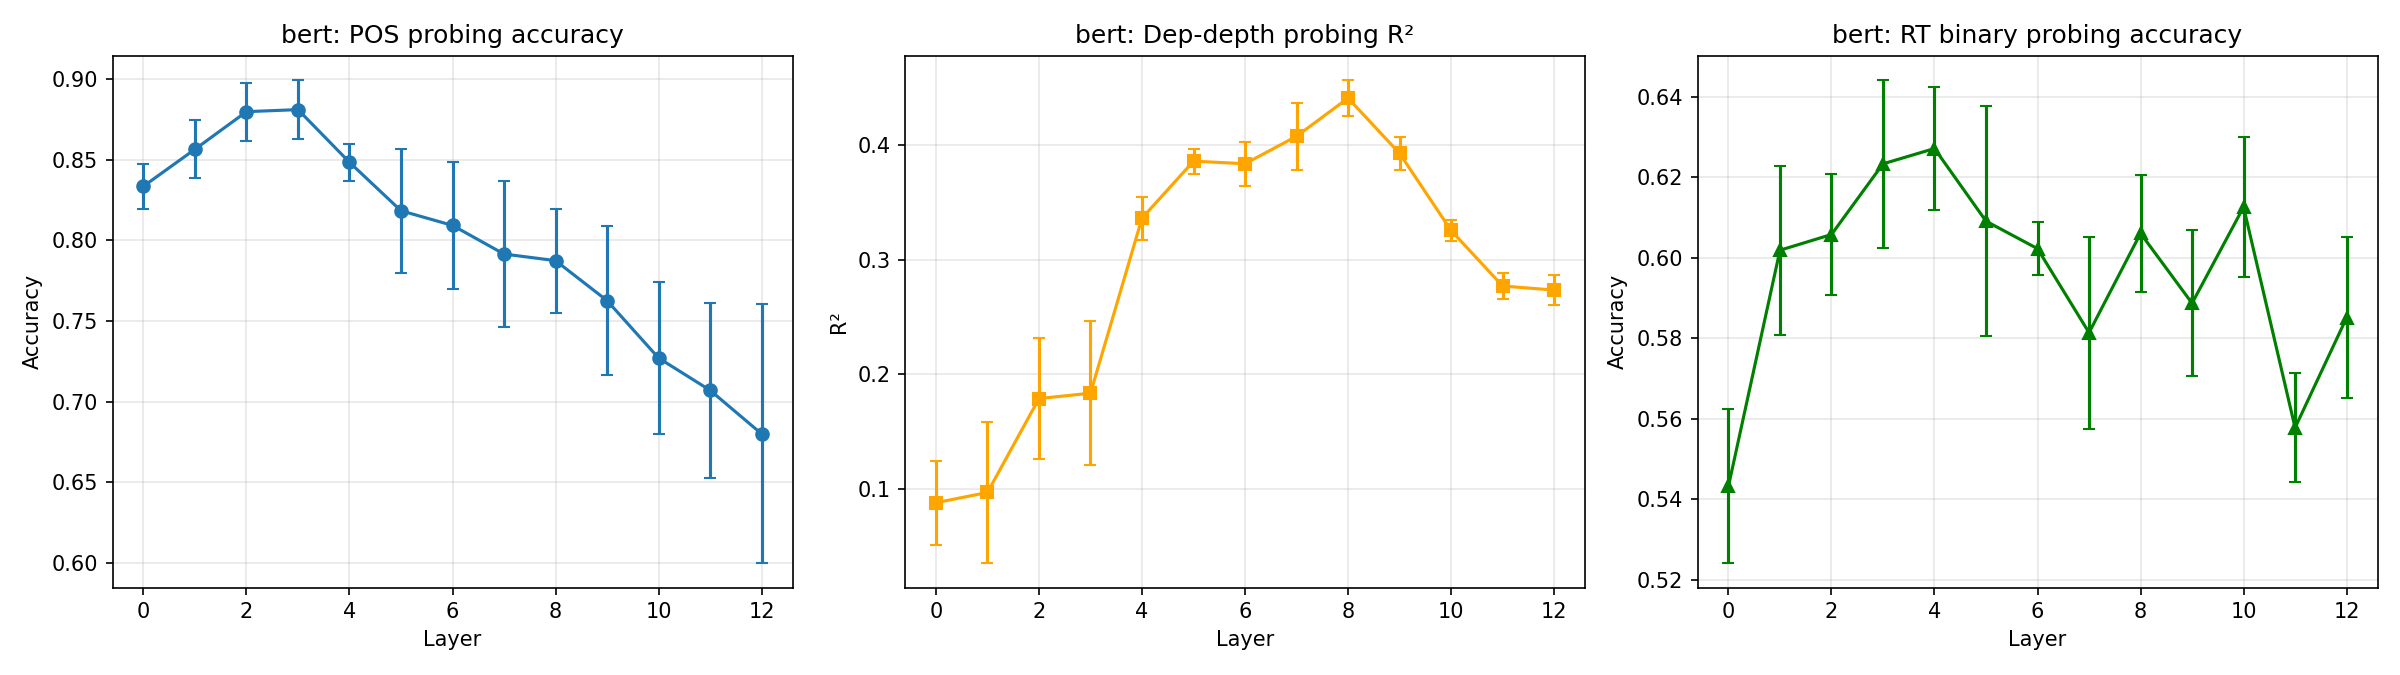
\includegraphics[width=\textwidth]{figures/bert_probing_curves.png}
    \caption{BERT}
    \label{fig:probing_bert}
\end{subfigure}
\vspace{0.3em}
\begin{subfigure}[t]{\textwidth}
    \centering
    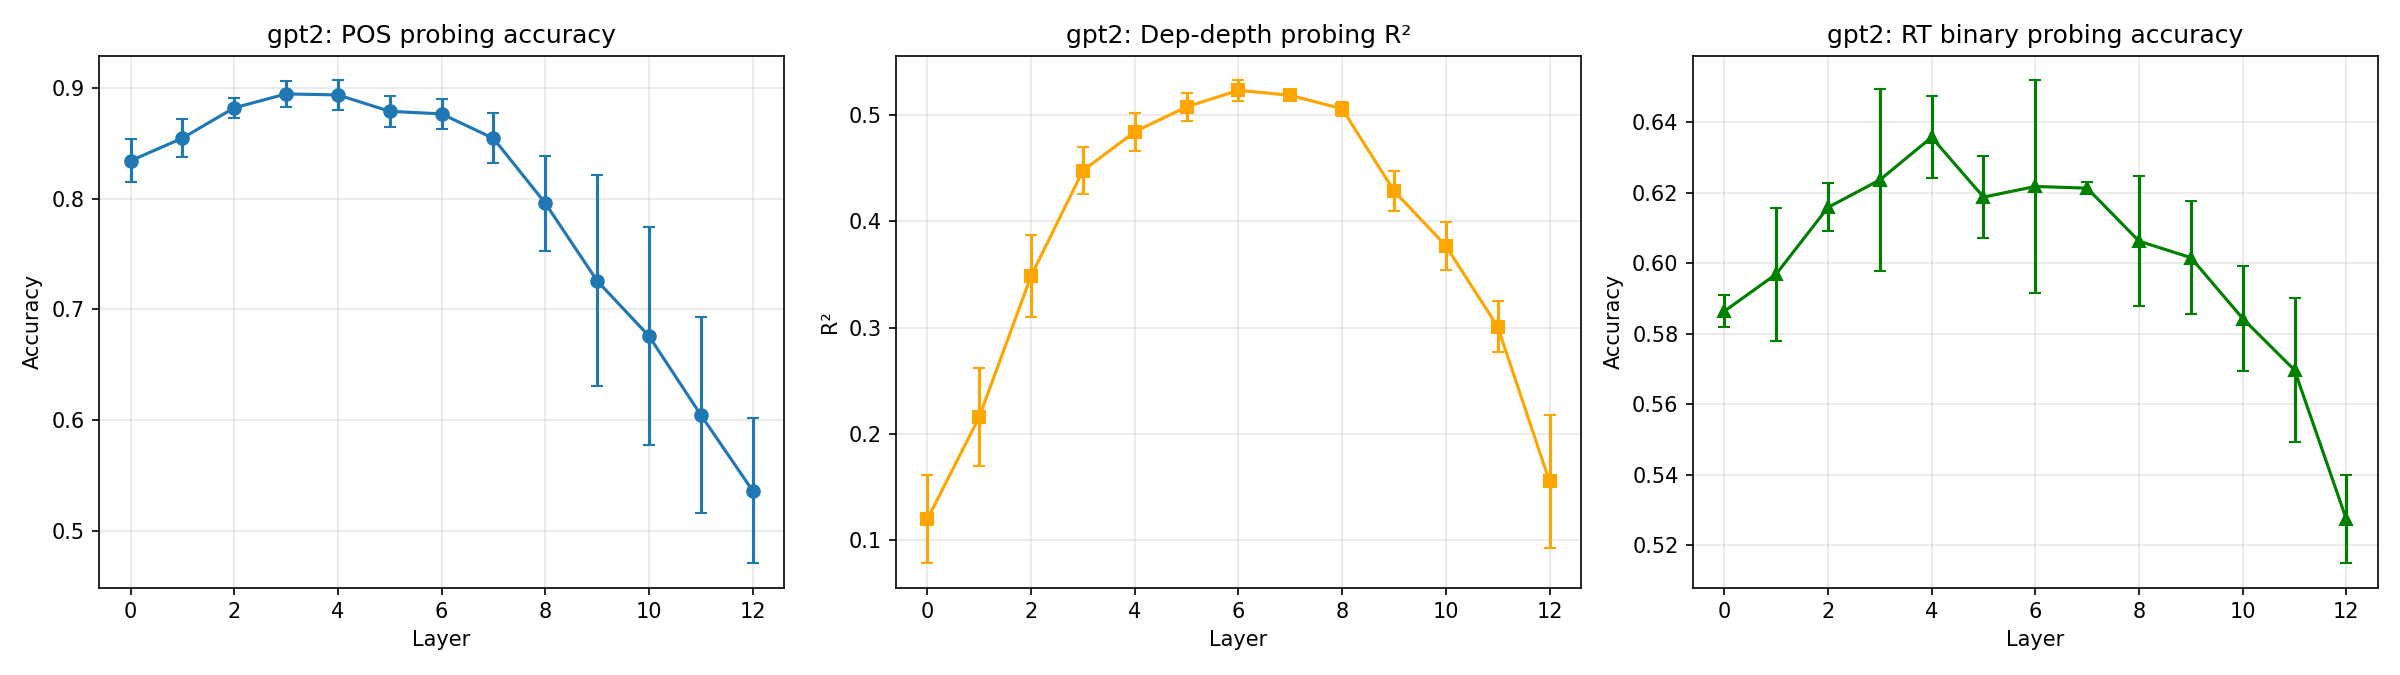
\includegraphics[width=\textwidth]{figures/gpt2_probing_curves.png}
    \caption{GPT-2}
    \label{fig:probing_gpt2}
\end{subfigure}
\caption{Layer-wise probing: POS accuracy (blue), dep-depth $R^2$ (orange), RT binary accuracy (green), $\pm 1$ SD across 3-fold CV. POS peaks early (L3--4), dep-depth peaks mid (BERT L8, GPT-2 L6), RT peaks at L4. GPT-2 shows steeper late-layer collapse for all three probes.}
\label{fig:probing}
\end{figure*}

\paragraph{Activation visualisation: POS tags.}
Figure~\ref{fig:pos} presents PCA and t-SNE projections of the best-layer embeddings coloured by POS tag.
In both models, t-SNE reveals well-separated clusters for major syntactic categories: nouns, verbs, determiners, adpositions, adjectives, and pronouns each form distinct groupings, with punctuation tokens clustering into tight, isolated islands.
The separation between function words (DET, ADP, PRON, AUX) and content words (NOUN, VERB, ADJ) is particularly striking; these two classes occupy largely non-overlapping regions of the t-SNE space.
The PCA projections show more diffuse structure: BERT L5 exhibits an annular (ring-shaped) geometry with POS categories distributed azimuthally, while GPT-2 L4 shows an elongated manifold with a function-to-content gradient along the first principal component.
The strong POS separability at these layers confirms that middle-layer representations carry rich syntactic information, consistent with the high probing accuracy ($>88\%$) at layers~3--4.

\begin{figure*}[t]
\centering
\begin{subfigure}[t]{\textwidth}
    \centering
    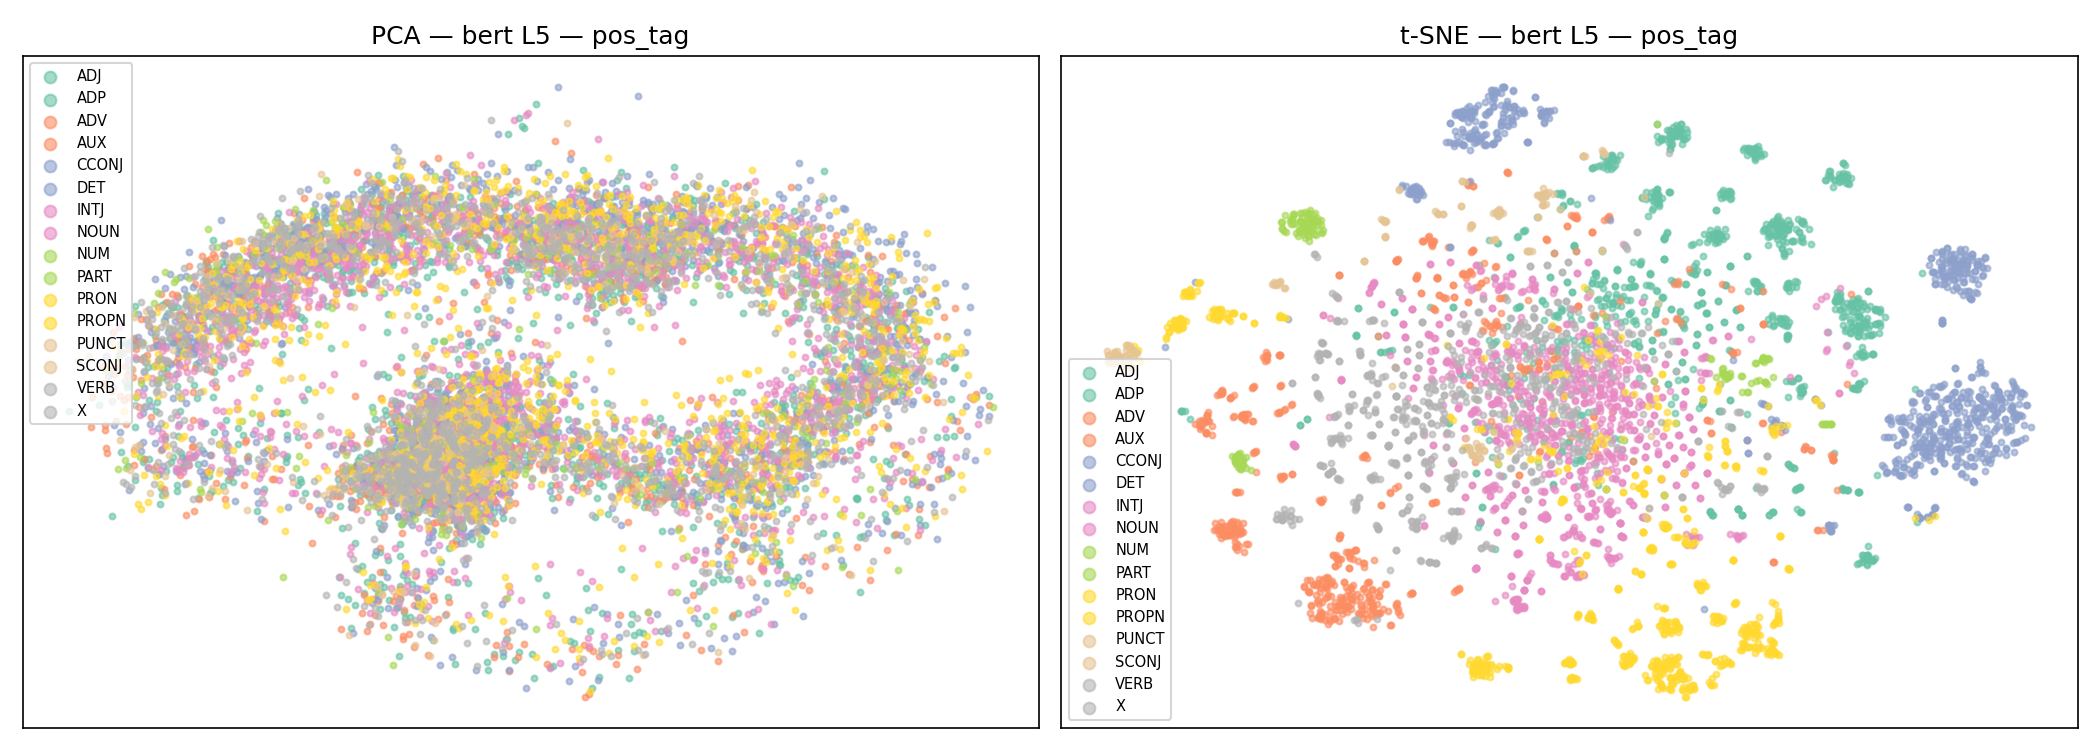
\includegraphics[width=\textwidth]{figures/pos_tag_L5.png}
    \caption{BERT L5: PCA reveals an annular structure; t-SNE separates 16 POS categories into distinct clusters, with PUNCT forming tight isolated groups and NOUN occupying the largest region.}
    \label{fig:pos_bert}
\end{subfigure}
\vspace{0.3em}
\begin{subfigure}[t]{\textwidth}
    \centering
    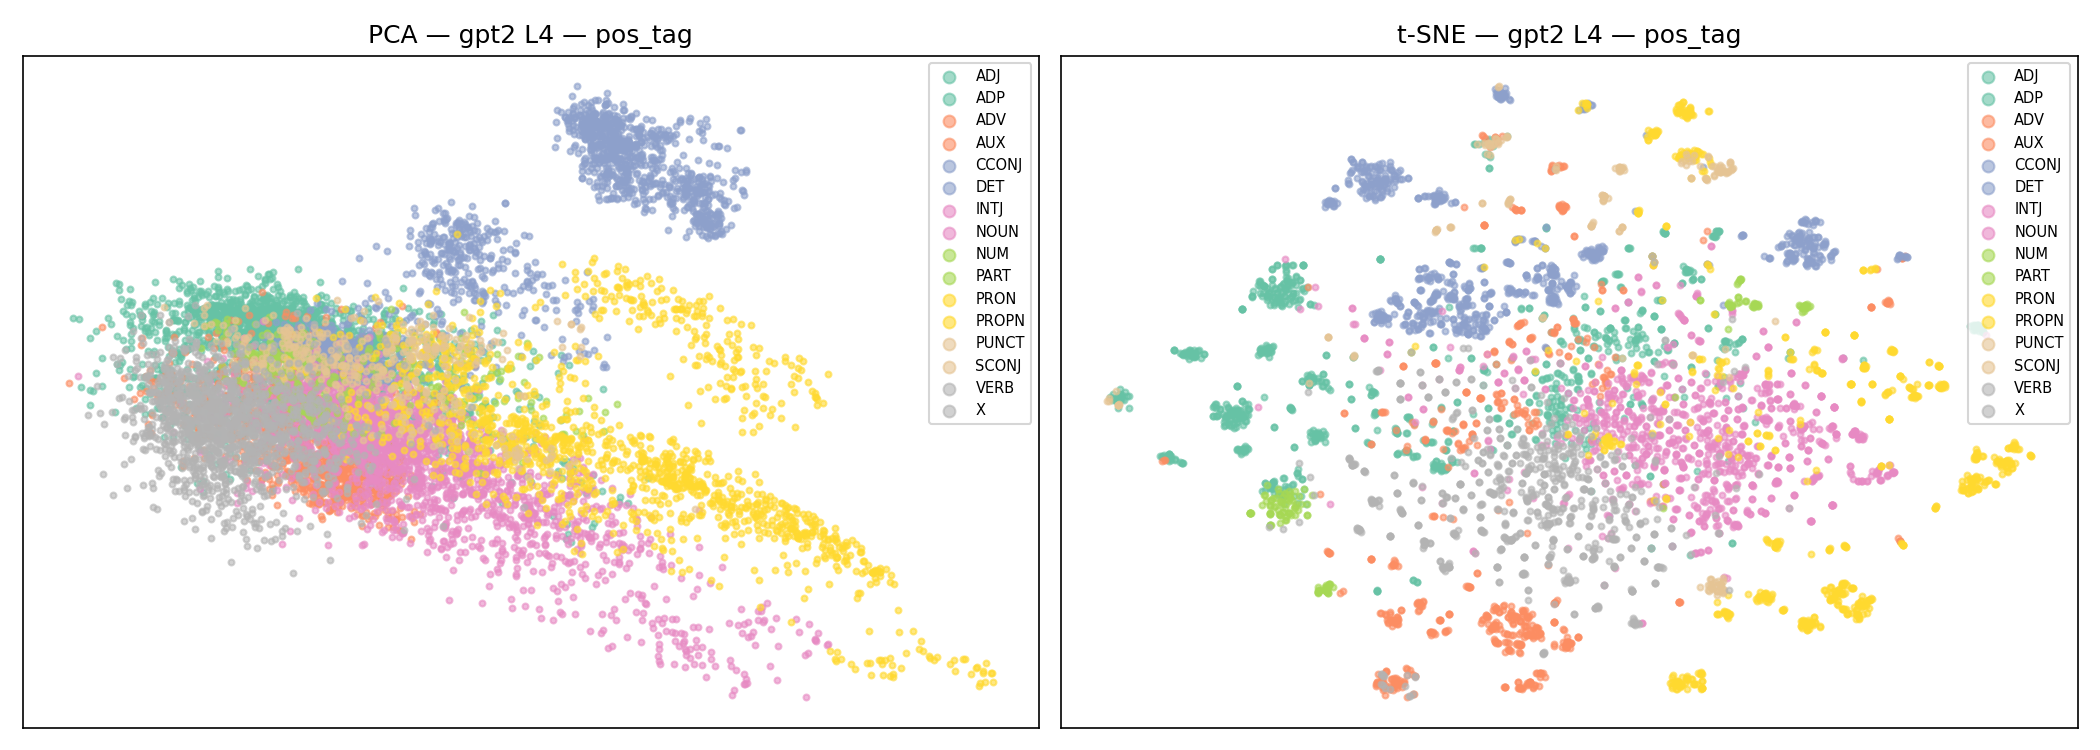
\includegraphics[width=\textwidth]{figures/pos_tag_L4.png}
    \caption{GPT-2 L4: PCA shows an elongated manifold with a function-word-to-content-word gradient; t-SNE clusters are comparably clean, with DET, ADP, and PRON forming particularly tight groups.}
    \label{fig:pos_gpt2}
\end{subfigure}
\caption{PCA (left half of each panel) and t-SNE (right half) projections of best-layer embeddings coloured by POS tag. Both models show clear syntactic clustering at their peak RT-predictive layers, with t-SNE revealing well-separated category islands.}
\label{fig:pos}
\end{figure*}

\paragraph{Additional activation overlays.}
Projections of the same embedding geometry coloured by reading-time quartile, surprisal quartile, and ambiguity region are presented in Appendix~\ref{app:viz}.
Unlike POS tags, RT quartiles produce a spatial gradient rather than discrete clusters, consistent with the moderate binary probing accuracy (${\sim}63\%$) and the influence of extra-linguistic factors (fatigue, motor noise) on reading times.
The surprisal gradient is markedly cleaner than the RT gradient, with high- and low-surprisal tokens occupying distinct regions of embedding space; in GPT-2's PCA, surprisal aligns with the primary axis of variation, confirming it as a dominant factor in middle-layer geometry.
Ambiguity-region overlays show onset and disambiguation tokens scattered uniformly among controls with no separable clustering, consistent with the null H1 result and indicating that these naturalistic garden-path structures are too mild to produce distinctive representational signatures.

\subsection{Cross-Dataset Validation}

We apply the full pipeline (feature extraction, layer-wise regression, and interpretability analysis) to the Dundee Eye-Tracking Corpus \citep{kennedy2003} using gaze duration as the dependent variable.
This extension tests whether the middle-layer advantage generalises from self-paced reading to eye-tracking, and from the narrative genre of Natural Stories to newspaper editorials.

% =========================================================================
\section{Discussion}

\paragraph{Why H2 succeeds.}
The middle-layer peak for reading-time prediction aligns with a growing body of evidence that intermediate transformer layers encode syntactic structure \citep{jawahar2019}.
Our probing results (Figure~\ref{fig:probing}) make this connection explicit: the layers that best predict reading times (BERT L5, GPT-2 L4) are precisely those that best encode dependency depth and POS information.
The visualisations reinforce this: POS tags are cleanly separable at these layers (Figure~\ref{fig:pos}), and RT quartiles show a spatial gradient aligned with the same representational geometry (Appendix~\ref{app:viz}, Figure~\ref{fig:rt}).
This suggests that reading difficulty is driven primarily by syntactic processing, and that the ``cognitively relevant'' representation lies at the interface between lexical encoding and task-specific abstraction.

The steeper late-layer degradation in GPT-2 (L12 test $R^2 = 0.148$) compared to BERT (L12 test $R^2 = 0.227$) reflects a training-objective asymmetry analysed in detail in \S4.1: GPT-2's causal objective drives final-layer representations toward narrative-specific predictions that overfit under story-level cross-validation, while BERT's bidirectional objective yields more transferable final-layer representations.
The probing results reinforce this: GPT-2's POS accuracy collapses to 53.6\% at layer~12 (vs.\ BERT's 68.0\%), and its dependency-depth $R^2$ falls to 0.155 (vs.\ BERT's 0.273), confirming that GPT-2's late layers sacrifice general syntactic encoding for prediction-specific information.

\paragraph{Why H1 is null.}
We deliberately tested H1 on naturalistic text to establish whether the causal-vs.-masked distinction produces detectable region-specific differences under ecologically valid conditions, before investing in controlled materials.
The null result is itself informative: the relative clauses and NP/S complements that arise in naturalistic narrative are predominantly low-ambiguity structures where readers rarely commit to a wrong parse, and the embedding geometry confirms this (Appendix~\ref{app:viz}, Figure~\ref{fig:ambiguity}): onset and disambiguation tokens are geometrically indistinguishable from controls.
Three factors jointly explain the null:
(1)~H1 requires strong garden-path sentences (e.g., ``the horse raced past the barn fell''), which are vanishingly rare in naturalistic text;
(2)~the small held-out sample (120 onset/disambiguation tokens) yields weak statistical power, requiring effect sizes of approximately 0.005~log-ms (${\approx}5$~ms reading time) before $p < 0.1$;
(3)~including surprisal as a regression feature absorbs much of the incremental-prediction signal that H1 predicts GPT-2 should uniquely capture, reducing the residual contrast to below detectable levels.
A targeted follow-up using the SyntaxGym test suite \citep{gauthier2020}, where onset--disambiguation contrasts are experimentally controlled and sample sizes are adequate, would provide a more decisive test.

\paragraph{Causal vs.\ masked surprisal.}
GPT-2 outperforms BERT at peak ($R^2$ 0.467 vs.\ 0.383), likely because causal surprisal is a stronger linear predictor of reading time than BERT's pseudo-log-likelihood estimate \citep{salazar2020}.
The surprisal quartile visualisation (Appendix~\ref{app:viz}, Figure~\ref{fig:surprisal}) supports this interpretation: surprisal is a dominant axis of variation in GPT-2's middle-layer geometry, with high- and low-surprisal tokens occupying distinct regions of the embedding space.
This advantage is not architectural per se but reflects the alignment between GPT-2's left-to-right training objective and the incremental nature of human reading.

% =========================================================================
\section{Conclusion}

We presented a systematic comparison of causal (GPT-2) and masked (BERT) language models for predicting human reading times, with three main findings.
First, middle layers of both models substantially outperform final layers for reading-time prediction (H2), and the same layers that best predict reading times also best encode syntactic features, establishing a mechanistic link between model representations and cognitive processing difficulty.
Second, the predicted region-specific advantage of causal models at ambiguity onset and masked models at disambiguation (H1) is directionally present but statistically undetectable in naturalistic text, calling for evaluation on controlled garden-path materials.
Third, GPT-2's overall advantage over BERT reflects the alignment between its left-to-right training objective and human incremental processing, rather than representational superiority at any specific depth.

Our pipeline (feature extraction, layer-wise regression, probing, and visualisation) extends to the Dundee Eye-Tracking Corpus and is fully reproducible.\footnote{Code and data: \url{https://github.com/bitmap4/cp-project}}
Future work should test H1 on experimentally controlled garden-path items and extend the layer-wise analysis to larger models (e.g., GPT-2 Medium/Large, RoBERTa) to test whether the middle-layer peak scales with model size.

% =========================================================================
\section*{Limitations}

Several limitations constrain the generalisability of our findings.
First, both GPT-2 and BERT-base are relatively small models (12 layers, 110--124M parameters); it is unknown whether the middle-layer peak persists, shifts, or sharpens in larger architectures (e.g., GPT-2 Medium/Large, RoBERTa-large).
Second, our H1 test is underpowered by design: the Natural Stories Corpus lacks experimentally controlled garden-path items, yielding only 120 onset and 120 disambiguation tokens in the held-out set.
A dedicated garden-path corpus such as SyntaxGym \citep{gauthier2020} is needed for a decisive test.
Third, linear probing may underestimate the true syntactic information encoded in each layer, as nonlinear decoders could recover additional structure; our results therefore represent a lower bound on layer-wise encoding.
Fourth, reading times are aggregated to per-token means across participants, discarding individual-level variation that may interact differently with causal and masked representations.
Finally, the automatic syntactic annotation via spaCy introduces noise in region boundaries, and the story-level train/test split, while preventing data leakage, limits the effective test-set size.

% =========================================================================
\section*{Ethics Statement}

This work uses two publicly available corpora (Natural Stories and Dundee) that were collected under institutional ethics approval by their respective creators.
We do not collect new human-subjects data.
Our models (GPT-2, BERT-base) are standard pretrained checkpoints used solely for representation extraction; we do not fine-tune or deploy them in any user-facing system.
The research poses no foreseeable risks beyond those inherent to computational psycholinguistics.

% =========================================================================

\bibliography{references}

% =========================================================================
\appendix
\section{Ridge Regression Hyperparameters}
\label{app:hyperparams}

The regularisation strength $\alpha$ was selected per layer from the grid $\{0.01, 0.1, 1.0, 10.0, 100.0, 1000.0\}$ by maximising validation-set $R^2$.
At peak-performance layers (BERT L5, GPT-2 L4), moderate $\alpha$ values were selected, reflecting well-conditioned representations.
At late layers, both models selected $\alpha = 1000$ (the maximum value in the grid), consistent with the severe overfitting documented in Table~\ref{tab:layerwise}: the optimizer requires maximal regularisation to constrain late-layer representations that have specialised away from general syntactic features.
All features (embeddings, surprisal, log word length, log corpus frequency, position) were standardised using training-set statistics prior to fitting.

\section{Additional Activation Visualisations}
\label{app:viz}

Figures~\ref{fig:rt}--\ref{fig:ambiguity} present PCA and t-SNE projections of the same best-layer embeddings as Figure~\ref{fig:pos}, coloured by reading-time quartile, surprisal quartile, and ambiguity region respectively.
The spatial geometries are identical to those in Figure~\ref{fig:pos}; only the colour overlays differ.

\begin{figure*}[t]
\centering
\begin{subfigure}[t]{\textwidth}
    \centering
    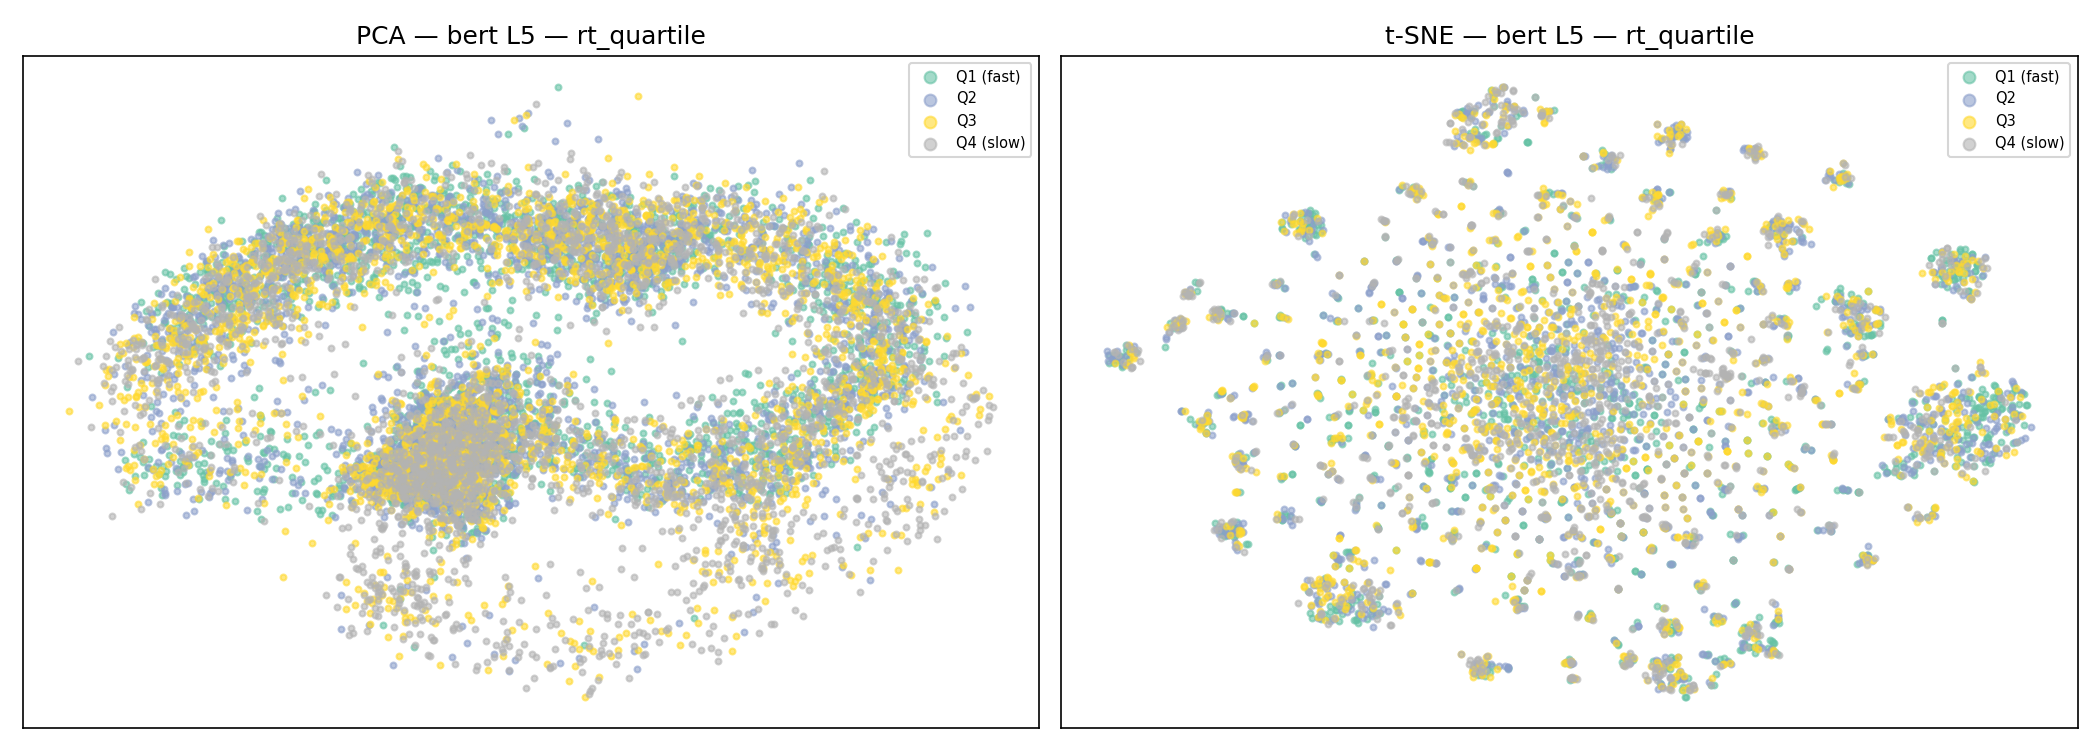
\includegraphics[width=\textwidth]{figures/rt_quartile_L5.png}
    \caption{BERT L5}
    \label{fig:rt_bert}
\end{subfigure}
\vspace{0.3em}
\begin{subfigure}[t]{\textwidth}
    \centering
    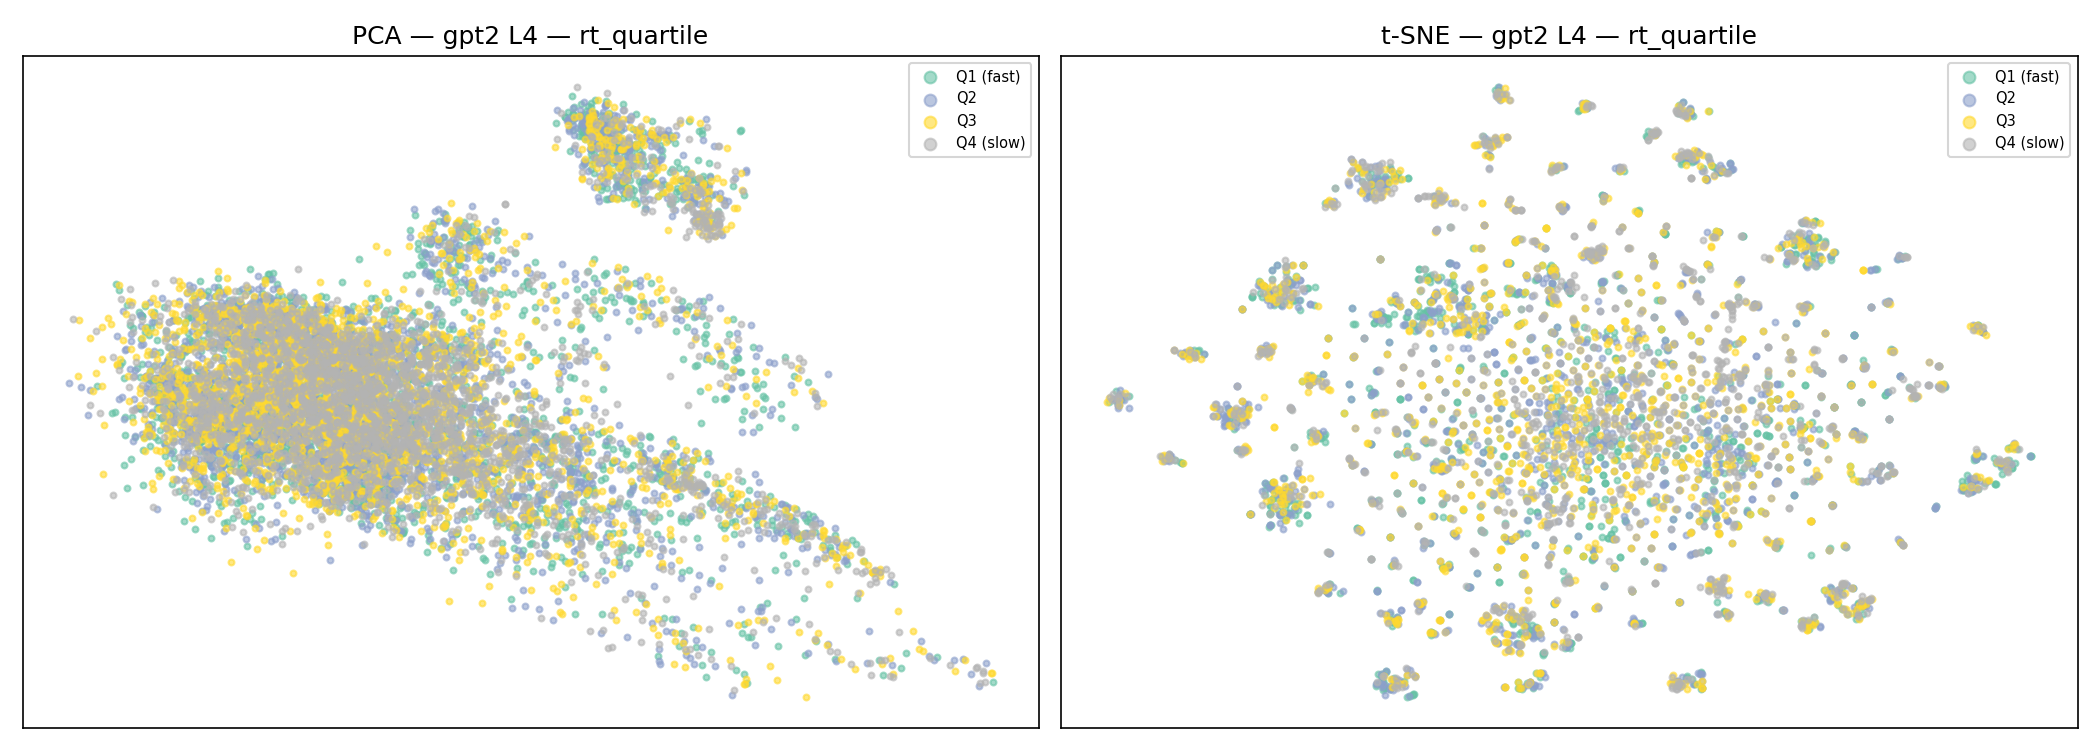
\includegraphics[width=\textwidth]{figures/rt_quartile_L4.png}
    \caption{GPT-2 L4}
    \label{fig:rt_gpt2}
\end{subfigure}
\caption{PCA and t-SNE projections coloured by reading-time quartile (Q1 = fast, Q4 = slow). RT quartiles produce a spatial gradient rather than discrete clusters, with GPT-2 showing more structured RT-homogeneous neighbourhoods.}
\label{fig:rt}
\end{figure*}

\begin{figure*}[t]
\centering
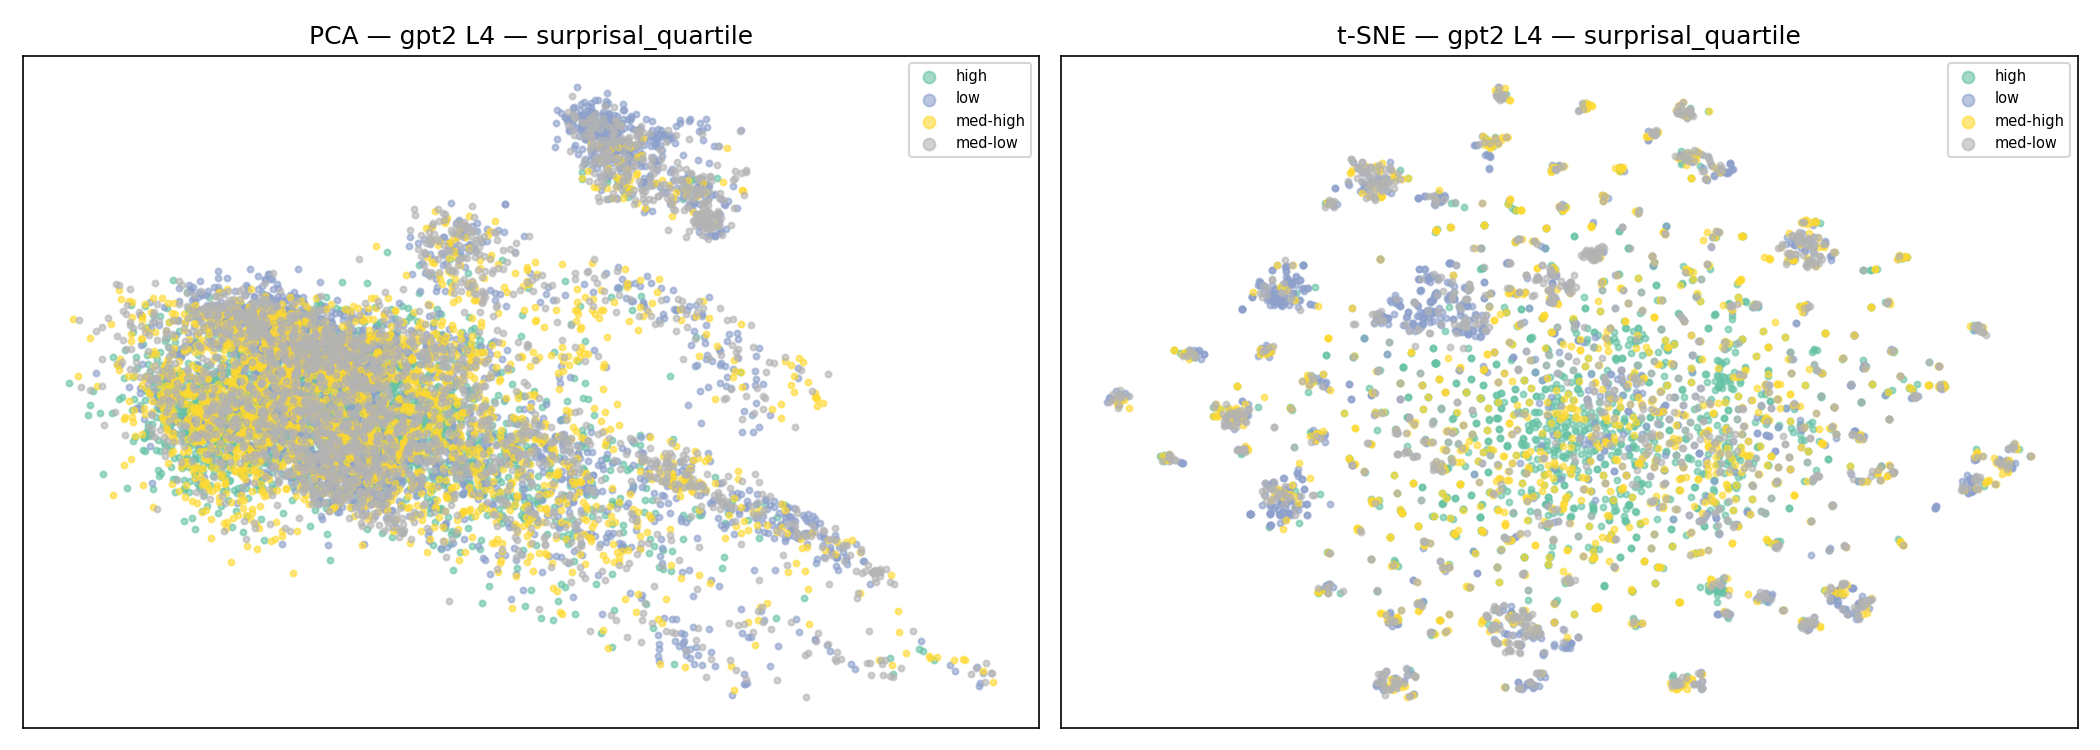
\includegraphics[width=\textwidth]{figures/surprisal_quartile_L4.png}
\caption{GPT-2 L4 embeddings coloured by surprisal quartile. PCA shows a clean gradient along PC1; t-SNE clusters high-surprisal tokens into distinct neighbourhoods. The surprisal structure is cleaner than the RT gradient (Figure~\ref{fig:rt_gpt2}), consistent with surprisal being a model-internal quantity.}
\label{fig:surprisal}
\end{figure*}

\begin{figure*}[t]
\centering
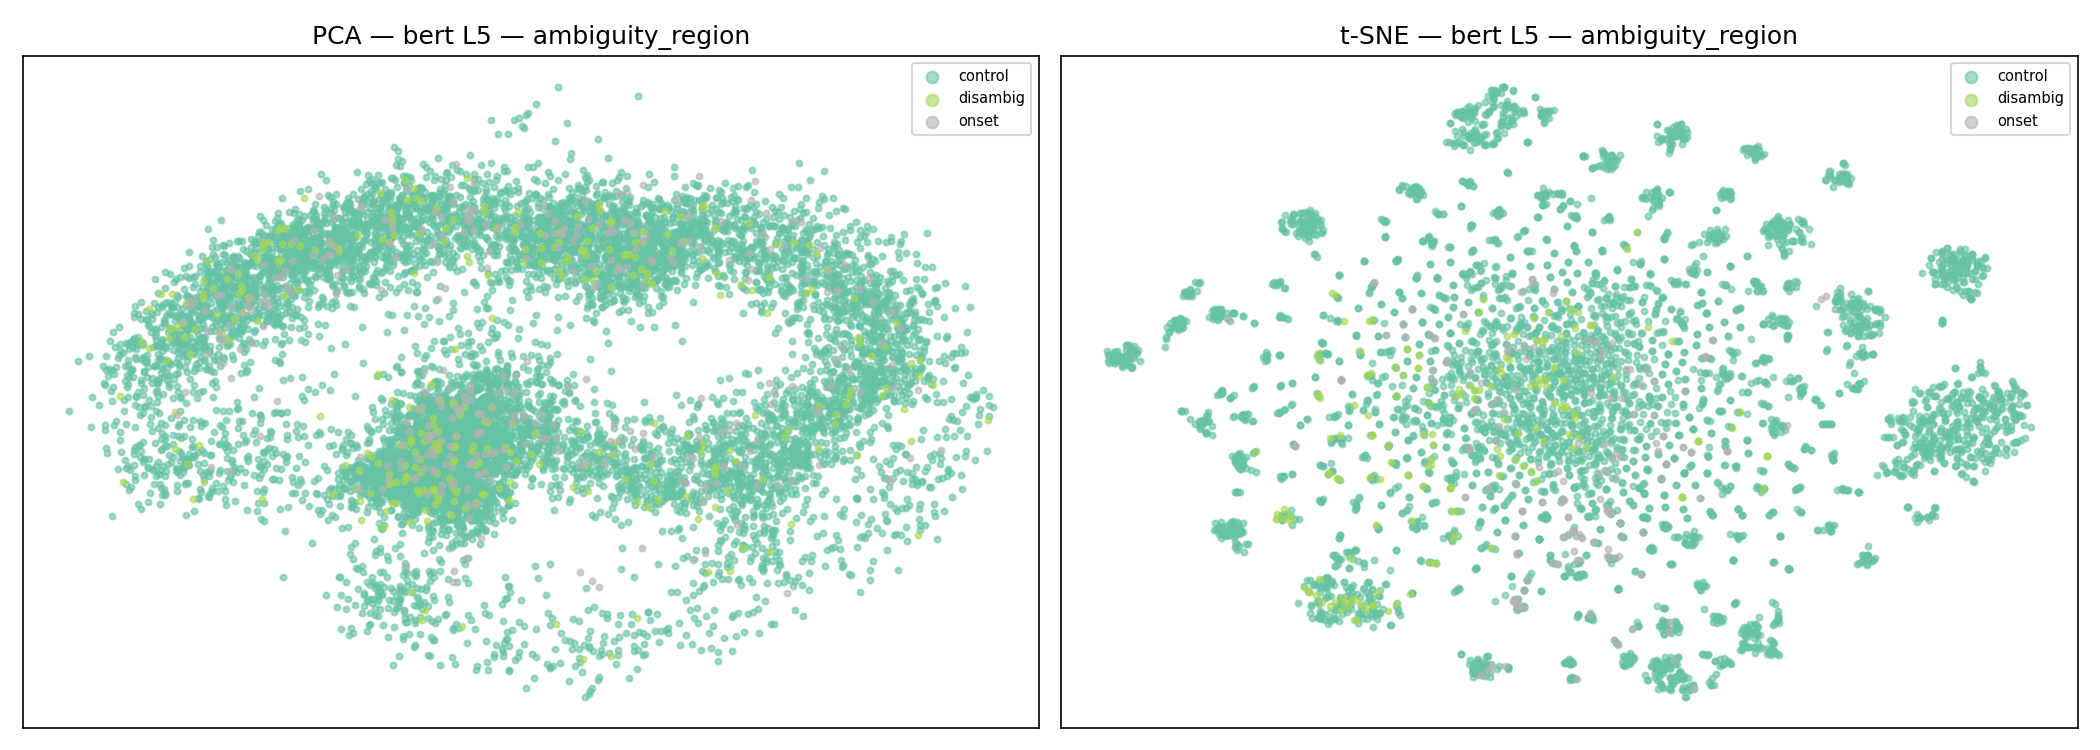
\includegraphics[width=\textwidth]{figures/ambiguity_region_L5.png}
\caption{BERT L5 embeddings coloured by syntactic region (onset, disambiguation, control). Onset and disambiguation tokens are uniformly dispersed among controls, consistent with the null H1 effect. GPT-2 L4 (not shown) displays the same pattern.}
\label{fig:ambiguity}
\end{figure*}

\end{document}
